\chapter{广度优先搜索}
当题目看不出任何规律,既不能用分治,贪心,也不能用动规时,这时候万能方法——搜索,
就派上用场了。搜索分为广搜和深搜,广搜里面又有普通广搜,双向广搜,A*搜索等。
深搜里面又有普通深搜,回溯法等。

广搜和深搜非常类似(除了在扩展节点这部分不一样),二者有相同的框架,如何表示状态?
如何扩展状态?如何判重?尤其是判重,解决了这个问题,基本上整个问题就解决了。


\section{算法框架} %%%%%%%%%%%%%%%%%%%%%%%%%%%%%%
\label{sec:bfs-template}


\subsubsection{适用场景}
注意,这里的总结是一种经验,一种概率,不是绝对的结论!

\textbf{输入数据}:没什么特征,不像深搜,需要有“递归”的性质。如果是树或者图,概率更大。

\textbf{状态转换图}:树或者图。

\textbf{求解目标}:求最短。


\subsubsection{思考的步骤}
\begin{enumerate}
\item 是求路径长度,还是路径本身(或动作序列)?
    \begin{enumerate}
    \item 如果是求路径长度,则状态里面要存路径长度
    \item 如果是求路径本身或动作序列
        \begin{enumerate}
            \item 要用一棵树存储宽搜过程中的路径
            \item 是否可以预估状态个数的上限?能够预估状态总数,则开一个大数组,用树的双亲表示法;如果不能预估状态总数,则要使用一棵通用的树(自己实现或用标准库)。这一步也是第4步的必要不充分条件。
        \end{enumerate}
    \end{enumerate}
\item 如何表示状态?即一个状态需要存储哪些些必要的数据,才能够完整提供如何扩展到下一步状态的所有信息。一般记录当前位置或整体局面。
\item 如何扩展状态?这一步跟第2步相关。状态里记录的数据不同,扩展方法就不同。对于固定不变的数据结构(一般题目直接给出,作为输入数据),如二叉树,图等,扩展方法很简单,直接往下一层走,对于隐式图,要先在第1步里想清楚状态所带的数据,想清楚了这点,那如何扩展就很简单了。
\item 关于判重,状态是否存在完美哈希方案?即将状态一一映射到整数,互相之间不会冲突。
    \begin{enumerate}
    \item 如果不存在,则需要使用通用的哈希表(自己实现或用标准库,例如\fn{std::unordered_set})来判重;自己实现哈希表的话,如果能够预估状态个数的上限,则可以开两个数组,head和next,表示哈希表,参考第 \S \ref{subsec:eightDigits}节方案2。
    \item 如果存在,则可以开一个大布尔数组,作为哈希表来判重,且此时可以精确计算出状态总数,而不仅仅是预估上限。
    \end{enumerate}
\end{enumerate}


\subsubsection{代码模板}
\begin{Codex}[label=bfs_template.c]
#include <stdio.h>
#include <string.h>

/***** 输入数据,用全局变量存放 *****/
...
/*
例如
int m = MAXN, n = MAXN;  // 迷宫的行数,列数
// 迷宫,0表示空地,1表示障碍物
int map[MAXN][MAXN];  // 迷宫,0表示空地,1表示障碍物
 */

/***** 一些常量 *****/
...
/* 例如
// 四个方向
const char name[4] = { 'U', 'R', 'D', 'L' };
const int dx[4] = { -1, 0, 1, 0 }; // 行
const int dy[4] = { 0, 1, 0, -1 }; // 列
*/

#ifndef __cplusplus
typedef char bool;
#define false 0
#define true 1
#endif

/**
 * @strut 状态
 */
typedef struct state_t {
    ... data1;  /** 状态的数据,可以有多个字段. */
    ... data2;  /** 状态的数据,可以有多个字段. */
    int action; /** 由父状态移动到本状态的动作,求动作序列时需要. */
    int index;  /** 本状态在path[]中的下标,求路径和动作序列时需要。
                    如果存在完美哈希,则不需要本字段(此时将
                   状态的哈希值作为下标,而哈希值可以直接计算出) */
    int father; /** 父状态在path[]中的下标,求路径或动作序列时需要 */
    int count;  /** 所花费的步骤数(也即路径长度-1),求路径长度时需要 */
} state_t;

/********** 如果题目要求输出路径或动作序列,则需要下面的变量和函数 ***********/

#define STATE_MAX ...  /* 状态总数 */
/**
 * 记录动作序列,树的双亲表示法.
 * 如果不能预估状态个数的上限,则不能用数组,要用通用树
 * 一般此时会有完美哈希方案,开一个大数组存储每个状态的动作,下标就是状态的哈希值
 * 其实一般用不了这么大的数组,广搜很很快就会结束
 */
state_t path[STATE_MAX];
int path_index = 0;  /** 每出现一个新状态,就增1,将状态存到该位置 */

/**
 * @brief 打印动作序列.
 * 如果有完美哈希方案,状态的哈希值就是下标。
 * 起点状态没有父亲和动作为-1,因为它没有父状态,也就没有所谓的从父节点到它的动作。
 * @param[in] end 终点状态的下标
 * @return 父状态
 */
void print_action(const int end) {
    if (path[end].father == -1) return;

    print_action(path[end].father);
    putchar(name[path[end].action]);
}

/**
 * @brief 打印坐标序列.
 * 如果有完美哈希方案,状态的哈希值就是下标。
 * 起点状态没有父亲和动作为-1,因为它没有父状态,也就没有所谓的从父节点到它的动作。
 * @param[in] end 终点状态的哈希值
 * @return 父状态
 */
void print_path(const int end) {
    if (path[end].father == -1) {
        printf("(%d, %d)\n", end / n, end % n);
        return;
    }
    print_path(path[end].father);
    printf("(%d, %d)\n", end / n, end % n);
}

/********** 如果题目要求输出路径或动作序列,则需要上面的变量和函数 ***********/

/** 计算状态的哈希值,如果存在完美哈希方案,则定义本函数,否则不需要.
 * 哈希值只依赖state_t的数据字段。
 */
int state_hash(const state_t *s);

/** 初始化查找表. */
void history_init();

/**
 * @brief 状态判重.
 * 一般用哈希表(set::unordered_set),如果存在完美哈希,则用数组
 * @param[in] s 状态
 * @return 已经访问过,返回true,否则false
 */
bool history_contains(const state_t *s);

/**
 * @brief 标记该状态已经被访问
 * @param[in] s 状态
 * @return 无
 */
void history_insert(const state_t *s);

/**
 * @brief 扩展第一个状态.
 * @param[in] s 状态
 * @param[out] next 第一个状态
 * @return 如果还有下一个状态,返回true,否则返回false
 */
void state_extend_init(const state_t *s);

/**
 * @brief 扩展下一个状态.
 * @param[in] s 状态
 * @param[out] next 下一个状态
 * @return 如果还有下一个状态,返回true,否则返回false
 */
bool state_extend(const state_t *s, state_t *next);

/**
 * @brief 判断状态是否为目标.
 * @param[in] s 状态
 * @return 如果已经达到目标状态,返回true,否则false
 */
bool state_is_target(const state_t *s);

typedef state_t queue_elem_t; // 元素的类型
/* 等价于复制粘贴,这里为了节约篇幅,使用include,在OJ上提交时请用复制粘贴 */
#include "queue.c"  /* 见“栈和队列->队列”这节,如果是C++,则使用std::queue */

/*
 * @brief 广搜
 *
 * @param[in] x 入口的x坐标
 * @param[in] y 入口的y坐标
 * @return 目标状态在path[]中的下标,如果不需要求路径,则声明为 void
 */
int bfs(state_t *start) {
    queue_t *q = queue_create(16);
    history_init();

    start->action = -1;   /* 起点状态没有动作 */
    start->index = path_index++;
    start->father = -1;   /* 起点状态没有父状态 */
    start->count = 0;

    path[state_hash(start) or start->index] = *start;
    history_insert(start); // 千万别忘记了标记此处的访问记录
    if (state_is_target(start)) /* 如果起点就是终点,返回 */
        return state_hash(start) or start->index;
    queue_push(q, *start);

    while (!queue_empty(q)) {
        const state_t s = queue_front(q);
        state_t next;
        queue_pop(q);

        state_extend_init(&s);
        while (state_extend(&s, &next)) {
            if (state_is_target(&next)) {
                // printf("%d\n", next.count);
                queue_destroy(q);
                return next.index or state_hash(&next);
            }
            queue_push(q, next);
            history_insert(&next);
        }
    }
    queue_destroy(q);
    return -1;
}

int main(void) {
    state_t start;
    int end; /* 目标状态在path[]中的下标 */
    input(&start);

    end = bfs(&start);

    print_action(end);
    printf("\n");
    print_path(end);
    return 0;
}

/************ functions implement ************/

/* 哈希表容量,要大于状态总数,若存在完美哈希方案,则等于状态总数 */
#define HASH_CAPACITY ...

/** 哈希表,标记状态是否已访问过。
 * 如果存在完美哈希方案,则用数组作为哈希表,否则用std::unordered_set
 */
... visited
// 例如 bool visited[HASH_MAX];

int state_hash(const state_t *s) {
    ...
}

void history_init() {
    /* 如果是数组 */
    memset(visited, 0, sizeof(visited));
    /* 如果是 std::unordered_set */
    visited.clear();
}

bool history_contains(const state_t *s) {
    /* 如果是数组 */
    return visited[state_hash(s)] == true;
    /* 如果是 std::unordered_set */
    return visited.count(s) > 0;
}

void history_insert(const state_t *s) {
    /* 如果是数组 */
    visited[state_hash(s)] = true;
    /* 如果是 std::unordered_set */
    visited.insert(s);
}

/** 扩展节点时,记录当前到了什么哪一步.
 * 是state_extend_init()和state_extend()的共享变量
 */
int action_cur;
/* 动作的范围 */
#define ACTION_BEGIN ...
#define ACTION_END ...

/* 扩展点的位置,是 state_extend_init()和state_extend()的共享变量 */
int extend_pos;

void state_extend_init(const state_t *s) {
    action_cur = ACTION_BEGIN;
    extend_pos = // 根据 s 进行计算
}

bool state_extend(const state_t *s, state_t *next) {
    // extract values from s
    value1 = ...
    value2 = ...
    while(action_cur < ACTION_END) {
        // apply action_cur to values
        value1 = ...
        value2 = ...
        next->count = s->count + 1;
        if (values are valid) {
            // assign new values to next's data fields
            next->data1 = value1
            next->data2 = value2

            if (!history_contains(next)) { /* 判重 */
                next->action = action_cur;
                next->index = path_index++;
                next->father = s->index or state_hash(s);
                /* 记录路径 */
                path[next->index or state_hash(next)] = *next;
                action_cur++;  /* return前别忘了增1 */
                return true;
            }
        }
        action_cur++;
    }
    return false;
}

// 目标状态
const state_t END = {..., 0};

bool state_is_target(const state_t *s) {
    ...
    /* 例如 return memcmp(s->data, END.data, xx * sizeof(yy) == 0; */
    /* 例如 return s->data == END.data; */
}
\end{Codex}

\section{走迷宫} %%%%%%%%%%%%%%%%%%%%%%%%%%%%%%

\subsubsection{描述}
一个迷宫由一个01矩阵表示,每个单元格要么是空地(用0表示),要
么是障碍物(用1表示)。你的任务是找到一条从入口到出口的最短路径。任何时候都不能在障碍物格子中,也不
能走到迷宫之外。只能横着走或竖着走,不能斜着走。数据保证有唯一解。

\subsubsection{输入}
一个$5 \times 5$的二维数组

\subsubsection{输出}
左上角到右下角的最短路径

\subsubsection{样例输入}
\begin{Code}
0 1 0 0 0
0 1 0 1 0
0 0 0 0 0
0 1 1 1 0
0 0 0 1 0
\end{Code}

\subsubsection{样例输出}
(0, 0)
(1, 0)
(2, 0)
(2, 1)
(2, 2)
(2, 3)
(2, 4)
(3, 4)
(4, 4)

\subsubsection{分析}
既然求的是“最短”,很自然的思路是用BFS。举个例子,在如下图所示的迷宫中,假设
入口是左上角$(0,0)$,我们就从入口开始用BFS遍历迷宫,就可以算出从入口到
所有点的最短路径(如图~\ref{fig:maze}(a)所示),以及这些路径上每个节点的
前驱(如图~\ref{fig:maze}(b)所示)。

\begin{center}
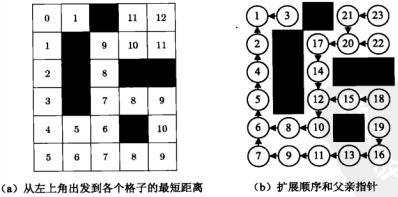
\includegraphics{maze.png}\\
\figcaption{用BFS求迷宫中最短路径}\label{fig:maze}
\end{center}

\subsubsection{代码}
\begin{Codex}[label=maze.c]
#include <stdio.h>
#include <string.h>

#define MAXN 5

// 迷宫的行数,列数
int m = MAXN, n = MAXN;
// 迷宫,0表示空地,1表示障碍物
int map[MAXN][MAXN];

// 四个方向
const char name[4] = { 'U', 'R', 'D', 'L' };
const int dx[4] = { -1, 0, 1, 0 }; // 行
const int dy[4] = { 0, 1, 0, -1 }; // 列

#ifndef __cplusplus
typedef char bool;
#define false 0
#define true 1
#endif

typedef struct state_t {
    int data;
    int action;
    int father;
} state_t;

#define STATE_MAX MAXN*MAXN  /* 状态总数 */

state_t path[STATE_MAX];

void print_action(const int end) {
    if (path[end].father == -1) return;

    print_action(path[end].father);
    putchar(name[path[end].action]);
}

void print_path(const int end) {
    if (path[end].father == -1) {
        printf("(%d, %d)\n", end / n, end % n);
        return;
    }
    print_path(path[end].father);
    printf("(%d, %d)\n", end / n, end % n);
}

int state_hash(const state_t *s);

void history_init();

bool history_contains(const state_t *s);

void history_insert(const state_t *s);

void state_extend_init(const state_t *s);

bool state_extend(const state_t *s, state_t *next);

bool state_is_target(const state_t *s);

typedef state_t queue_elem_t; // 元素的类型
/* 等价于复制粘贴,这里为了节约篇幅,使用include,在OJ上提交时请用复制粘贴 */
#include "queue.c"  /* 见“栈和队列->队列”这节,如果是C++,则使用std::queue */

int bfs(state_t *start) {
    queue_t *q = queue_create(16);
    history_init();

    start->action = -1;
    start->father = -1;

    path[state_hash(start)] = *start;
    history_insert(start);
    if (state_is_target(start))
        return state_hash(start);
    queue_push(q, *start);

    while (!queue_empty(q)) {
        const state_t s = queue_front(q);
        queue_pop(q);
        state_t next;
        state_extend_init(&s);
        while (state_extend(&s, &next)) {
            if (state_is_target(&next)) {
                queue_destroy(q);
                return state_hash(&next);
            }
            queue_push(q, next);
            history_insert(&next);
        }
    }
    queue_destroy(q);
    return -1;
}

int main(void) {
    int i, j;
    state_t start = {0, -1, -1}; /* 左上角为起点 */
    int end;

    for (i = 0; i < m; i++) {
        for (j = 0; j < n; j++) {
            scanf("%d", &map[i][j]);
        }
    }

    end = bfs(&start);
    print_path(end);
    return 0;
}

/********** functions implement **************/
/* 哈希表容量,要大于状态总数,若存在完美哈希方案,则等于状态总数 */
#define HASH_CAPACITY STATE_MAX
bool visited[HASH_CAPACITY];

int state_hash(const state_t *s) {
    return s->data;
}

void history_init() {
    memset(visited, 0, sizeof(visited));
}

bool history_contains(const state_t *s) {
    return visited[state_hash(s)] == true;
}

void history_insert(const state_t *s) {
    visited[state_hash(s)] = true;
}

int action_cur;
#define ACTION_BEGIN 0
#define ACTION_END 4
/** 扩展点,即当前位置 */
int x, y;

void state_extend_init(const state_t *s) {
    action_cur = ACTION_BEGIN;
    x = s->data / n;
    y = s->data % n;
}

bool state_extend(const state_t *s, state_t *next) {
    while(action_cur < ACTION_END) {
        const int nx = x + dx[action_cur];
        const int ny = y + dy[action_cur];

        if (nx >= 0 && nx < m && ny >= 0 && ny < n && !map[nx][ny]) {
            next->data = nx * n + ny;

            if (!history_contains(next)) { /* 判重 */
                /* 记录路径 */
                next->action = action_cur;
                next->father = state_hash(s);
                path[state_hash(next)] = *next;

                action_cur++;  /* return前别忘了增1 */
                return true;
            }
        }
        action_cur++;
    }
    return false;
}

const state_t END = {24, -1, -1};
bool state_is_target(const state_t *s) {
    return s->data == END.data;
}
\end{Codex}

\subsubsection{相关的题目}
与本题相同的题目:
\begindot
\item 《算法竞赛入门经典》\footnote{刘汝佳,算法竞赛入门经典,清华大学出版社,2009}第108页6.4.2节
\item  POJ 3984 迷宫问题, \myurl{http://poj.org/problem?id=3984}
\myenddot

与本题相似的题目:
\begindot
\item  POJ 2049 Finding Nemo, \myurl{http://poj.org/problem?id=2049}
\myenddot


\section{八数码问题} %%%%%%%%%%%%%%%%%%%%%%%%%%%%%%
\label{subsec:eightDigits}

\subsubsection{描述}
编号为1$\sim$8的8个正方形滑块摆成3行3列,有一个格子空着,如图~\ref{fig:eightDigits}所示。

\begin{center}
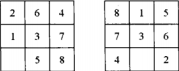
\includegraphics{eight-digits.png}\\
\figcaption{用BFS求迷宫中最短路径}\label{fig:eightDigits}
\end{center}

每次可以把与空格相邻的滑块(有公共边才算相邻)移到空格中,而它原
来的位置就成了新的空格。目标局面固定如下(用$x$表示空格):
\begin{Code}
1 2 3
4 5 6
7 8 x
\end{Code}

给定初始局面,计算出最短的移动路径。

\subsubsection{输入}
用一行表示一个局面,例如下面的这个局面:
\begin{Code}
 1  2  3
 x  4  6
 7  5  8
\end{Code}
可以表示为 1 2 3 x 4 6 7 5 8。 

\subsubsection{输出}
如果有解答,输出一个由四个字母'r','l','u','d'组成的移动路径。
如果没有,输出"unsolvable"。 

\subsubsection{样例输入}
\begin{Code}
2  3  4  1  5  x  7  6  8
\end{Code}

\subsubsection{样例输出}
\begin{Code}
ullddrurdllurdruldr
\end{Code}

\subsubsection{分析}
计算“最短”,很自然的想到BFS。

如何表示一个状态?一个3*3的棋盘,首先可以想到用一个数组\fn{int data[9]}来表示。把每个格子看做是整数的一位的话,可以用一个整数来表示,最大的棋盘87654321x,表示成整数就是876543210,没有超过32位整数的范围。

如何判重?用哈希表,自己实现或者用STL。C++ STL 里有\fn{std::set}, C++ 11新加入了\fn{std::unordered_set}。建议先用STL写一个版本,确保主算法正确,然后把\fn{std::set}(或\fn{std::unordered_set})替换成自己写的哈希表。

由于本题的特殊性,存在一种完美哈希(perfect hashing)方案。即\textbf{康托展开}。棋盘本身是一个排列,将排列转化为序数,用序数作为hash值。例如,1,2,3 这三个数字的全排列,按字典序,依次为
\begin{Code}
123 -- 0
132 -- 1
213 -- 2
231 -- 3
312 -- 4
321 -- 5
\end{Code}
其中,左侧为排列,右侧为其序数。

此题更优的解法还有双向BFS(见\S \ref{sec:biBFS}),A*算法(见\S \ref{sec:astar})。

\subsubsection{代码}

方案1,完美哈希,使用康托展开。

\begin{Codex}[label=eight_digits_bfs.c]
/* POJ 1077 Eight, http://poj.org/problem?id=1077 */
#include <stdio.h>
#include <string.h>

#define DIGITS 9 // 棋盘中数字的个数,也是变进制数需要的位数
#define     MATRIX_EDGE 3       // 棋盘边长

/***** 一些常量 *****/
const int SPACE_NUMBER = 0; // 空格对应着数字 0
// 上下左右四个方向
const int dx[] = {-1, 1, 0, 0};
const int dy[] = {0, 0, -1, 1};
const char name[] = { 'u', 'd', 'l', 'r' };

#ifndef __cplusplus
typedef char bool;
#define false 0
#define true 1
#endif

typedef char int8_t;

/**
 * @strut 状态
 */
typedef struct state_t {
    int8_t data[DIGITS];  /** 状态的数据. */
    int action; /* 由父状态移动到本状态的动作 */
    int father; /* 父状态在path[]中的下标,也即父状态的哈希值 */
    int count;  /** 所花费的步骤数(也即路径长度-1) */
} state_t;

// 3x3的棋盘,状态最多有 9!种
#define STATE_MAX 362880  /* 状态总数 */

state_t path[STATE_MAX+1];

/**
 * @brief 打印动作序列.
 * @param[in] end 终点状态的哈希值
 * @return 父状态
 */
void print_action(const int end) {
    if (path[end].father == -1) return;

    print_action(path[end].father);
    putchar(name[path[end].action]);
}

int state_hash(const state_t *s);

void history_init();

bool history_contains(const state_t *s);

void history_insert(const state_t *s);

void state_extend_init(const state_t *s);

bool state_extend(const state_t *s, state_t *next);

bool state_is_target(const state_t *s);

typedef state_t queue_elem_t; // 元素的类型
/* 等价于复制粘贴,这里为了节约篇幅,使用include,在OJ上提交时请用复制粘贴 */
#include "queue.c"  /* 见“栈和队列->队列”这节,如果是C++,则使用std::queue */

int bfs(state_t *start) {
    queue_t *q = queue_create(16);
    history_init();

    start->action = -1;
    start->father = -1;
    start->count = 0;

    path[state_hash(start)] = *start;
    history_insert(start);
    if (state_is_target(start))
        return state_hash(start);
    queue_push(q, *start);

    while (!queue_empty(q)) {
        const state_t s = queue_front(q);
        state_t next;
        queue_pop(q);

        state_extend_init(&s);
        while (state_extend(&s, &next)) {
            if (state_is_target(&next)) {
                // printf("%d\n", next.count);
                queue_destroy(q);
                return state_hash(&next);
            }
            queue_push(q, next);
            history_insert(&next);
        }
    }
    queue_destroy(q);
    return -1;
}

/**
 * @brief 输入.
 * @return 无
 */
void input(state_t *start) {
    int ch, i;
    for (i = 0; i < DIGITS; ++i) {
        do {
            ch = getchar();
        } while ((ch != EOF) && ((ch < '1') || (ch > '8')) && (ch != 'x'));
        if (ch == EOF) return;
        if (ch == 'x') start->data[i] = 0; // x 映射成数字 0
        else           start->data[i] = ch - '0';
    }
}

/** for wikioi 1225 */
void input1(state_t *start) {
    int i, n;
    scanf("%d", &n);

    /* 将整数转化为棋盘 */
    for(i = DIGITS-1; i >= 0; i--) {
        start->data[i] = n % 10;
        n /= 10;
    }
}

int main(void) {
    state_t start;
    int end; /* 目标状态在path[]中的下标 */
    input(&start);

    end = bfs(&start);

    print_action(end);
    printf("\n");
    return 0;
}

/********** functions implement **************/

/********** 方案1,完美哈希,使用康托展开 **************/

// 9 位变进制数(空格)能表示0到(9!-1)内的所有自然数,恰好有9!个,
// 与状态一一对应,因此可以把状态一一映射到一个9位变进制数

// 9 位变进制数,每个位数的单位,0!~8!
const int fac[] = {40320, 5040, 720, 120, 24, 6, 2, 1, 1};
/* 哈希表容量,要大于状态总数,若存在完美哈希方案,则等于状态总数 */
#define HASH_CAPACITY STATE_MAX

bool visited[HASH_CAPACITY];

int state_hash(const state_t *s) {
    int i, j;
    int key = 0;
    for (i = 0; i < DIGITS; i++) {
        int cnt = 0;  /* 逆序数 */
        for (j = i + 1; j < DIGITS; j++) if (s->data[i] > s->data[j]) cnt++;
        key += fac[i] * cnt;
    }
    return key;
}

void history_init() {
    memset(visited, 0, sizeof(visited));
}

bool history_contains(const state_t *s) {
    return visited[state_hash(s)] == true;
}

void history_insert(const state_t *s) {
    visited[state_hash(s)] = true;
}

int action_cur;
#define ACTION_BEGIN 0
#define ACTION_END 4

/* 扩展点,即0的位置 */
int z;

void state_extend_init(const state_t *s) {
    action_cur = ACTION_BEGIN;
    for (z = 0; z < DIGITS; z++) {
        if (s->data[z] == SPACE_NUMBER) {
            break;  // 找 0 的位置
        }
    }
}

bool state_extend(const state_t *s, state_t *next) {
    const int x = z / MATRIX_EDGE; // 行
    const int y = z % MATRIX_EDGE; // 列

    while (action_cur < ACTION_END) {
        const int newx = x + dx[action_cur];
        const int newy = y + dy[action_cur];
        const int newz = newx * MATRIX_EDGE + newy;

        if (newx >= 0 && newx < MATRIX_EDGE && newy >= 0 &&
                newy < MATRIX_EDGE) { // 没有越界
            *next = *s;
            next->data[newz] = SPACE_NUMBER;
            next->data[z] = s->data[newz];
            next->count = s->count + 1;
            if (!history_contains(next)) { /* 判重 */
                next->action = action_cur;
                next->father = state_hash(s);
                /* 记录路径 */
                path[state_hash(next)] = *next;
                action_cur++; /* return前别忘了增1 */
                return true;
            }
        }
        action_cur++;
    }
    return false;
}

// 目标状态
const state_t END = {{1, 2, 3, 4, 5, 6, 7, 8, 0}, -1, -1};
// for wikioi 1225
const state_t END1 = {{1, 2, 3, 8, 0, 4, 7, 6, 5}, -1, -1};

bool state_is_target(const state_t *s) {
    return memcmp(s->data, END.data, DIGITS * sizeof(int8_t)) == 0;
}
\end{Codex}

方案2,不知道是否存在完美哈希方案,但能够预估状态个数的上限,用树双亲表示法存储路径,用自己实现的哈希表判重。

\begin{Codex}[label=eight_digits_bfs2.c]
/* POJ 1077 Eight, http://poj.org/problem?id=1077 */
#include <stdio.h>
#include <string.h>
#include <assert.h>

#define DIGITS 9 // 棋盘中数字的个数,也是变进制数需要的位数
#define     MATRIX_EDGE 3       // 棋盘边长

/***** 一些常量 *****/
const int SPACE_NUMBER = 0; // 空格对应着数字 0
// 上下左右四个方向
const int dx[] = {-1, 1, 0, 0};
const int dy[] = {0, 0, -1, 1};
const char name[] = { 'u', 'd', 'l', 'r' };

#ifndef __cplusplus
typedef char bool;
#define false 0
#define true 1
#endif

typedef char int8_t;

/**
 * @strut 状态
 */
typedef struct state_t {
    int8_t data[DIGITS];  /** 状态的数据. */
    int action; /* 由父状态移动到本状态的动作 */
    int index;  /** 本状态在path[]中的下标 */
    int father; /** 父状态在path[]中的下标 */
    int count;  /** 所花费的步骤数(也即路径长度-1) */
} state_t;

// 3x3的棋盘,状态最多有 9!种
#define STATE_MAX 362880  /* 状态总数 */

state_t path[STATE_MAX+1];
int path_index = 0;

/**
 * @brief 打印动作序列.
 * @param[in] end 终点状态的哈希值
 * @return 父状态
 */
void print_action(const int end) {
    if (path[end].father == -1) return;

    print_action(path[end].father);
    putchar(name[path[end].action]);
}

void history_init();

bool history_contains(const state_t *s);

void history_insert(const state_t *s);

void state_extend_init(const state_t *s);

bool state_extend(const state_t *s, state_t *next);

bool state_is_target(const state_t *s);

typedef state_t queue_elem_t; // 元素的类型
/* 等价于复制粘贴,这里为了节约篇幅,使用include,在OJ上提交时请用复制粘贴 */
#include "queue.c"  /* 见“栈和队列->队列”这节,如果是C++,则使用std::queue */

int bfs(state_t *start) {
    queue_t *q = queue_create(16);
    history_init();

    start->action = -1;
    start->index = path_index++;
    start->father = -1;
    start->count = 0;

    path[start->index] = *start;
    history_insert(start);
    if (state_is_target(start))
        return state_hash(start);
    queue_push(q, *start);

    while (!queue_empty(q)) {
        const state_t s = queue_front(q);
        state_t next;
        queue_pop(q);

        state_extend_init(&s);
        while (state_extend(&s, &next)) {
            if (state_is_target(&next)) {
                // printf("%d\n", next.count);
                queue_destroy(q);
                return next.index;
            }
            queue_push(q, next);
            history_insert(&next);
        }
    }
    queue_destroy(q);
    return -1;
}

/**
 * @brief 输入.
 * @return 无
 */
void input(state_t *start) {
    int ch, i;
    for (i = 0; i < DIGITS; ++i) {
        do {
            ch = getchar();
        } while ((ch != EOF) && ((ch < '1') || (ch > '8')) && (ch != 'x'));
        if (ch == EOF) return;
        if (ch == 'x') start->data[i] = 0; // x 映射成数字 0
        else           start->data[i] = ch - '0';
    }
}

/** for wikioi 1225 */
void input1(state_t *start) {
    int i, n;
    scanf("%d", &n);

    /* 将整数转化为棋盘 */
    for(i = DIGITS-1; i >= 0; i--) {
        start->data[i] = n % 10;
        n /= 10;
    }
}

int main(void) {
    state_t start;
    int end;
    input(&start);

    end = bfs(&start);

    print_action(end);
    printf("\n");
    return 0;
}

/********** functions implement **************/

/********** 方案2 不知道完美哈希方案,自己实现哈希表 **************/
#define HASH_CAPACITY  10000000  /* 哈希表容量,要大于状态总数 */

int head[HASH_CAPACITY];
int next[STATE_MAX];

int state_hash(const state_t *s) {
    int i;
    int ret = 0;
    for(i = 0; i < DIGITS; i++) ret = ret * 10 + s->data[i];
    return ret % HASH_CAPACITY;
}

void history_init() {
    memset(head, 0, sizeof(head));
    memset(next, 0, sizeof(next));
}

bool history_contains(const state_t *s) {
    const int h = state_hash(s);
    int u = head[h]; // 从表头开始查找单链表
    while(u) {
        // 找到了
        if(memcmp(path[u].data, s->data,
                DIGITS * sizeof(int8_t)) == 0) return true;
        u = next[u]; // 顺着链表继续找
    }
    return false;
}

void history_insert(const state_t *s) {
    const int h = state_hash(s);
    int u = head[h]; // 从表头开始查找单链表
    while(u) {
        // 找到了,插入失败
        if(memcmp(path[u].data, path[s->index].data,
                sizeof(DIGITS * sizeof(int8_t))) == 0) return;
        u = next[u]; // 顺着链表继续找
    }
    assert(head[h] >= 0);
    next[s->index] = head[h];  /* 插入到首节点前面,头查法 */
    head[h] = s->index;
    return;
}

int action_cur;
#define ACTION_BEGIN 0
#define ACTION_END 4

/* 扩展点,即0的位置 */
int z;

void state_extend_init(const state_t *s) {
    action_cur = ACTION_BEGIN;
    for (z = 0; z < DIGITS; z++) {
        if (s->data[z] == SPACE_NUMBER) {
            break;  // 找 0 的位置
        }
    }
}

bool state_extend(const state_t *s, state_t *next) {
    const int x = z / MATRIX_EDGE; // 行
    const int y = z % MATRIX_EDGE; // 列

    while (action_cur < ACTION_END) {
        const int newx = x + dx[action_cur];
        const int newy = y + dy[action_cur];
        const int newz = newx * MATRIX_EDGE + newy;

        next->count = s->count + 1;
        if (newx >= 0 && newx < MATRIX_EDGE && newy >= 0 &&
                newy < MATRIX_EDGE) { // 没有越界
            *next = *s;
            next->data[newz] = SPACE_NUMBER;
            next->data[z] = s->data[newz];

            if (!history_contains(next)) { /* 判重 */
                next->action = action_cur;
                next->index = path_index++;
                next->father = s->index;
                /* 记录路径 */
                path[next->index] = *next;
                action_cur++; /* return前别忘了增1 */
                return true;
            }
        }
        action_cur++;
    }
    return false;
}

// 目标状态
const state_t END = {{1, 2, 3, 4, 5, 6, 7, 8, 0}, -1, -1};
// for wikioi 1225
const state_t END1 = {{1, 2, 3, 8, 0, 4, 7, 6, 5}, -1, -1};

bool state_is_target(const state_t *s) {
    return memcmp(s->data, END.data, DIGITS * sizeof(int8_t)) == 0;
}
\end{Codex}

方案3,不知道完美哈希方案,但能够预估状态个数的上限制,用树双亲表示法存储路径,用标准库的哈希表判重。

\begin{Codex}[label=eight_digits_bfs3.cpp]
//前面的代码与方案2一摸一样
//...

/********** 方案3 不知道完美哈希方案,使用标准库的哈希表 **************/

// 重载 state_t 的 == 操作符
typedef struct state_t {
    int8_t data[DIGITS];  /** 状态的数据. */
    int action; /* 由父状态移动到本状态的动作 */
    int index;  /** 本状态在path[]中的下标 */
    int father; /** 父状态在path[]中的下标 */
    int count;  /** 所花费的步骤数(也即路径长度-1) */

    bool operator==(const state_t& other) const {
        return memcmp(data, other.data, DIGITS * sizeof(int8_t)) == 0;
    }
} state_t;

#include <unordered_set>

// 定制一个哈希函数
namespace std {
template<> struct hash<state_t> {
    size_t operator()(const state_t & x) const {
        int i;
        int ret = 0;
        for (i = 0; i < DIGITS; i++)
            ret = ret * 10 + x.data[i];
        return ret;
    }
};
}

std::unordered_set<state_t> visited;

void history_init() {
    visited.clear();
}

bool history_contains(const state_t *s) {
    return visited.count(*s) > 0;
}

void history_insert(const state_t *s) {
    visited.insert(*s);
}

//...
//后面的代码也与方案2一摸一样
\end{Codex}

\subsubsection{相关的题目}
与本题相同的题目:
\begindot
\item 《算法竞赛入门经典》\footnote{刘汝佳,算法竞赛入门经典,清华大学出版社,2009} 第131页7.5.3节
\item  POJ 1077 Eight, \myurl{http://poj.org/problem?id=1077}
\item  wikioi 1225 八数码难题, \myurl{http://www.wikioi.com/problem/1225/}
\myenddot

与本题相似的题目:
\begindot
\item  POJ 2893 M × N Puzzle, \myurl{http://poj.org/problem?id=2893}
\myenddot


\section{四子连棋} %%%%%%%%%%%%%%%%%%%%%%%%%%%%%%

\subsubsection{描述}
在一个4*4的棋盘上摆放了14颗棋子,其中有7颗白色棋子,7颗黑色棋子,有两个空白地带,任何一颗黑白
棋子都可以向上下左右四个方向移动到相邻的空格,这叫行棋一步,黑白双方交替走棋,任意一方可以先走,
如果某个时刻使得任意一种颜色的棋子形成四个一线(包括斜线),这样的状态为目标棋局。

\subsubsection{输入}
一个4*4的初始棋局,黑棋子用B表示,白棋子用W表示,空格地带用O表示。

\subsubsection{输出}
移动到目标棋局的最少步数。

\subsubsection{样例输入}
\begin{Code}
BWBO
WBWB
BWBW
WBWO
\end{Code}

\subsubsection{样例输出}
\begin{Code}
5
\end{Code}

\subsubsection{分析}
求最少步数,很自然的想到广搜。

如何表示一个状态?用一个二维数组\fn{int board[4][4]}表示,还需要记录该状态是由白子还是黑子移动而导致的,走到该状态已经花费的步数。

如何扩展节点?每一步,从队列弹出一个状态,两个空格都可以向四个方向扩展,把得到的状态入队列。

如何判重?棋盘用二维矩阵存储,用0表示空格,1表示黑色,2表示白色,所以最后可以看成一个16位的三进制数。
用这个数作为棋盘的编码,就可以用来判重了。注意,本题要黑白交替走,所以我们要区分状态是由白子还是黑子移动而导致的。

可以用C++的\fn{std::map}来判重,
\begin{Code}
/* history[0]记录白子的历史,history[1]记录黑子的历史. */
std::map<int, bool> history[2];
\end{Code}

也可以开一个大数组当做哈希表,
\begin{Code}
#define HASH_MOD 43036875 /* hash表大小 */
/* history[0]记录白子的历史,history[1]记录黑子的历史. */
bool history[2][HASH_MOD];
\end{Code}

\subsubsection{代码}
\begin{Codex}[label=four_adjacent.c]
/** wikioi 1004 四子连棋  , http://www.wikioi.com/problem/1004 */
#include <stdio.h>
#include <string.h>

#define LEN 4   /* 边长 */

/* 右,左,上,下(左下角为坐标原点)*/
const int dx[] = { 1, -1, 0, 0 };
const int dy[] = { 0, 0, 1, -1 };


#ifndef __cplusplus
typedef char bool;
#define false 0
#define true 1
#endif

/**
 * @strut 状态
 */
typedef struct state_t {
    // 状态的数据
    int board[LEN][LEN]; /* 棋局,1表示黑子,2表示白子,0表示空白 */
    int color; /* 本状态是由白子还是黑子移动而导致的 */
    int count;  /** 所花费的步骤数(也即路径长度-1),求路径长度时需要 */
} state_t;

/**
 * @brief 计算状态的哈希值。
 * 棋盘用二维矩阵存储,用0表示空格,1表示黑色,2表示白色,所以最后可以看成
 * 一个16位的三进制数。最大为
 * 2222
 * 2221
 * 1111
 * 1100
 * 值为 43036875。
 * @return 棋盘所表示的三进制数转化为十进制数
 */
//TODO:共C16 7×C9 2个状态,用类似康托的方法储存
int state_hash(const state_t *s);

void history_init();

bool history_contains(const state_t *s);

void history_insert(const state_t *s);

void state_extend_init(const state_t *s);

bool state_extend(const state_t *s, state_t *next);

bool state_is_target(const state_t *s);

typedef state_t queue_elem_t; // 元素的类型
/* 等价于复制粘贴,这里为了节约篇幅,使用include,在OJ上提交时请用复制粘贴 */
#include "queue.c"  /* 见“栈和队列->队列”这节,如果是C++,则使用std::queue */

void bfs(state_t *start) {
    queue_t *q = queue_create(16);
    history_init();

    start->count = 0;
    start->color = 1;

    history_insert(start);
    queue_push(q, *start);

    start->color = 2;

    history_insert(start); // 千万别忘记了标记此处的访问记录
    if (state_is_target(start)) /* 如果起点就是终点,返回 */
        return;
    queue_push(q, *start);

    while (!queue_empty(q)) {
        const state_t s = queue_front(q);
        state_t next;
        queue_pop(q);

        state_extend_init(&s);
        while (state_extend(&s, &next)) {
            if (state_is_target(&next)) {
                printf("%d\n", next.count);
                queue_destroy(q);
                return;
            }
            queue_push(q, next);
            history_insert(&next);
        }
    }
    queue_destroy(q);
}

int main() {
    int i, j;
    char s[LEN + 1];
    state_t start;

    for (i = 0; i < LEN; i++) {
        scanf("%s", s);
        for (j = 0; j < LEN; j++) {
            if (s[j] == 'B') start.board[i][j] = 1;
            else if (s[j] == 'W') start.board[i][j] = 2;
            else start.board[i][j] = 0;
        }
    }

    bfs(&start);
    queue_destroy(q);
    return 0;
}

/************ functions implement ************/

/* 哈希表容量,要大于状态总数,若存在完美哈希方案,则等于状态总数 */
#define HASH_CAPACITY 43036875

/** 哈希表,标记状态是否已访问过。
 * visited[0]记录白子的历史,visited[1]记录黑子的历史.
 */
bool visited[2][HASH_CAPACITY];

#define RADIX 3 /* 三进制 */

int state_hash(const state_t *s) {
    int i, j;
    int ret = 0;

    for (i = 0; i < LEN; i++) {
        for (j = 0; j < LEN; j++) {
            ret = ret * RADIX + s->board[i][j];
        }
    }
    return ret;
}

void history_init() {
    memset(visited[0], 0, sizeof(sizeof(bool) * HASH_CAPACITY));
    memset(visited[1], 0, sizeof(sizeof(bool) * HASH_CAPACITY));
}

bool history_contains(const state_t *s) {
    return visited[s->color - 1][state_hash(s)] == true;
}

void history_insert(const state_t *s) {
    visited[s->color - 1][state_hash(s)] = true;
}

/* 扩展的时候,先定空格,再定方向 */
/* 记录当前方向,例如action_cur[0]记录了第一个空格,当前在扩展哪个方向
 */
int action_cur[2];
#define ACTION_BEGIN 0
#define ACTION_END 4

typedef struct point_t {
    int x, y;
} point_t;

/* 记录当前在扩展哪一个空格,值为0或1 */
int space_cur;
/* 两个空格的位置 */
point_t extend_pos[2];

void state_extend_init(const state_t *s) {
    int i, j, k;
    action_cur[0] = ACTION_BEGIN;
    action_cur[1] = ACTION_BEGIN;
    space_cur = 0;

    k = 0;
    // 寻找两个空白的格子的位置
    for (i = 0; i < LEN; i++) {
        for (j = 0; j < LEN; j++) {
            if (s->board[i][j] == 0) {
                extend_pos[k].x = i;
                extend_pos[k].y = j;
                k++;
            }
        }
    }
}

bool state_extend(const state_t *s, state_t *next) {
    int i;

    for (i = 0; i < 2; i++) { /* 先第一个空格,再第二个空格 */
        while (action_cur[i] < ACTION_END) {
            const int x = extend_pos[i].x;
            const int y = extend_pos[i].y;
            int nextx = x + dx[action_cur[i]];
            int nexty = y + dy[action_cur[i]];
            *next = *s;
            next->count = s->count + 1;
            next->color = 3 - s->color;

            if (nextx >= 0 && nextx < LEN && nexty >= 0 && nexty < LEN
                    /* 必须黑白交替走 */
                    && next->color == s->board[nextx][nexty]) {
                /* swap */
                {
                    int temp = next->board[x][y];
                    next->board[x][y] = next->board[nextx][nexty];
                    next->board[nextx][nexty] = temp;
                }

                if (!history_contains(next)) { /* 判重 */
                    action_cur[i]++; /* return前别忘了增1 */
                    return true;
                }
            }
            action_cur[i]++;
        }
    }
    return false;
}

bool state_is_target(const state_t *s) {
    int i, j;
    for (i = 0; i < LEN; i++) {  /* 逐行检查 */
        int flag = 1;  /* 某一行全是同一颜色 */
        for (j = 1; j < LEN; j++)
            if (s->board[i][j - 1] != s->board[i][j])
                flag = 0;
        if (flag)
            return 1;
    }
    for (j = 0; j < LEN; j++) { //逐列检查
        int flag = 1;  /* 某一行全是同一颜色 */
        for (i = 1; i < LEN; i++)
            if (s->board[i][j] != s->board[i - 1][j]) flag = 0;
        if (flag) return 1;
    }
    /* 斜线 */
    if (s->board[0][0] == s->board[1][1] && s->board[1][1] == s->board[2][2]
            && s->board[2][2] == s->board[3][3])
        return 1;
    if (s->board[0][3] == s->board[1][2] && s->board[1][2] == s->board[2][1]
            && s->board[2][1] == s->board[3][0])
        return 1;
    return 0;
}
\end{Codex}

\subsubsection{相关的题目}
与本题相同的题目:
\begindot
\item  wikioi 1004 四子连棋, \myurl{http://www.wikioi.com/problem/1004/}
\myenddot

与本题相似的题目:
\begindot
\item  None
\myenddot


\section{双向BFS} %%%%%%%%%%%%%%%%%%%%%%%%%%%%%%
\label{sec:biBFS}


\subsection{八数码问题}
题目见 \S \ref{subsec:eightDigits}。

\subsubsection{代码}

\begin{Codex}[label=eight_digits_bibfs.c]

\end{Codex}


\section{A*算法} %%%%%%%%%%%%%%%%%%%%%%%%%%%%%%
\label{sec:astar}

\textbf{A*算法 = 宽搜 + 优先队列}

将广搜模板(见第\S \ref{sec:bfs-template}节)中的队列改为优先队列,设计好当前状态距离目标状态的预估距离$h()$,就变成了A*算法!

\subsection{八数码问题}
题目见 \S \ref{subsec:eightDigits}。

\subsubsection{代码}
\begin{Codex}[label=eight_digits_astar.c]
/** POJ 1077 Eight, http://poj.org/problem?id=1077
 简单解释几个要点,便于理解代码.
1. 怎么判断是否有解?只要计算出的逆序个数总和为奇数,该数据必然无解
2. 如何判断某一状态是否到过?本题存在一种完美哈希方案,即用康托展开。
        详见 http://128kj.iteye.com/blog/1699795
3.使用优先队列,即堆,加速挑选最优值。
4.函数 g=此状态在搜索树中已经走过的路径的节点数.
5.估价函数 h ,采用曼哈顿距离, 见代码 calcH 函数。曼哈顿距离的定义是,
 假设有两个点(x1,y1),(x2,y2),则曼哈顿距离L1=|x1-x2| + |y1-y2|
 */
#include <stdio.h>
#include <string.h>

#define DIGITS 9 // 棋盘中数字的个数,也是变进制数需要的位数
#define     MATRIX_EDGE 3       // 棋盘边长
#define RADIX 10

/***** 一些常量 *****/
const int SPACE_NUMBER = 0; // 空格对应着数字 0
// 上下左右四个方向
const int dx[] = {-1, 1, 0, 0};
const int dy[] = {0, 0, -1, 1};
const char name[] = { 'u', 'd', 'l', 'r' };

// 目标状态
const int GOAL = 123456780;
// 每个数字在棋盘中的位置,例如0,在(2,2)=8这个位置上
int GOAL_POS[DIGITS];

#ifndef __cplusplus
typedef char bool;
#define false 0
#define true 1
#endif

/**
 * @strut 状态
 */
typedef struct state_t {
    int board;  /** 状态的数据,即棋局. */
    int action; /* 由父状态移动到本状态的动作 */
    int father; /* 父状态在path[]中的下标,也即父状态的哈希值 */
    int count;  /** 所花费的步骤数(也即路径长度-1),作为g */
    int h; /** 距离目标状态的估算距离 */
} state_t;

// 3x3的棋盘,状态最多有 9!种
#define STATE_MAX 362880  /* 状态总数 */

state_t path[STATE_MAX+1];

/**
 * @brief 打印动作序列.
 * @param[in] end 终点状态的哈希值
 * @return 父状态
 */
void print_action(const int end) {
    if (path[end].father == -1) return;

    print_action(path[end].father);
    putchar(name[path[end].action]);
}

int state_hash(const state_t *s);

void history_init();

bool history_contains(const state_t *s);

void history_insert(const state_t *s);

void state_extend_init(const state_t *s);

bool state_extend(const state_t *s, state_t *next);

bool state_is_target(const state_t *s);

typedef state_t heap_elem_t; // 元素的类型
/** 状态的比较函数 */
int cmp_state(const state_t *x, const state_t *y) {
    return (x->count + x->h) - (y->count + y->h);
}

/* 等价于复制粘贴,这里为了节约篇幅,使用include,在OJ上提交时请用复制粘贴 */
#include "heap.c"  /* 见“树->堆”这节 */

/**
 * 距离目标状态的估算距离h。
 * @param s 状态
 * @return h
 */
static int state_get_h(const state_t *state) {
    int i;
    int h = 0;
    int s = state->board;

    for (i = DIGITS - 1; i >= 0; --i) {
        const int p = s % RADIX;
        s /= RADIX;
        /* 曼哈顿距离 */
        h += abs(i / MATRIX_EDGE - GOAL_POS[p] / MATRIX_EDGE) +
            abs(i % MATRIX_EDGE - GOAL_POS[p] % MATRIX_EDGE);
    }
    return h;
}

/* 计算 GOAL_POS */
static void calc_goal_pos() {
    int cur = GOAL;
    int i;
    for (i = DIGITS-1; i >= 0 ; i--) {
        int digit = cur % RADIX;
        GOAL_POS[digit] = i;
        cur /= RADIX;
    }
}

int bfs(state_t *start) {
    heap_t *q = heap_create(16, cmp_state); /* 优先队列 */
    calc_goal_pos();
    history_init();

    start->action = -1;
    start->father = -1;
    start->count = 0;
    start->h = state_get_h(start);

    path[state_hash(start)] = *start;
    history_insert(start);
    if (state_is_target(start))
        return state_hash(start);
    heap_push(q, *start);

    while (!heap_empty(q)) {
        const state_t s = heap_top(q);
        state_t next;
        heap_pop(q);

        state_extend_init(&s);
        while (state_extend(&s, &next)) {
            if (state_is_target(&next)) {
                // printf("%d\n", next.count);
                heap_destroy(q);
                return state_hash(&next);
            }
            heap_push(q, next);
            history_insert(&next);
        }
    }
    heap_destroy(q);
    return -1;
}

static void int_to_board(int n, int board[DIGITS]) {
    int i;
    for (i = DIGITS - 1; i >= 0; i--) {
        board[i] = n % RADIX;
        n /= RADIX;
    }
}

static int board_to_int(const int board[DIGITS]) {
    int i, s = 0;
    for (i = 0; i < DIGITS; i++)
        s = s * RADIX + board[i];
    return s;
}

/**
 * @brief 输入.
 * @return 无
 */
void input(state_t *start) {
    int ch, i;
    int board[DIGITS];
    for (i = 0; i < DIGITS; ++i) {
        do {
            ch = getchar();
        } while ((ch != EOF) && ((ch < '1') || (ch > '8')) && (ch != 'x'));
        if (ch == EOF) return;
        if (ch == 'x') board[i] = 0; // x 映射成数字 0
        else           board[i] = ch - '0';
    }
    start->board = board_to_int(board);
}

/** for wikioi 1225 */
void input1(state_t *start) {
    scanf("%d", &start->board);
}

/**
 * 计算一个排列的逆序数,0 除外.
 */
static int inversion_count(int permutation) {
    int i, j;
    int d[DIGITS];
    int c = 0; // 逆序数

    for(i = DIGITS - 1; i >=0; i--) {
        d[i] = permutation % RADIX;
        permutation /= RADIX;
    }

    for (i = 1; i < DIGITS; i++)  if (d[i] != SPACE_NUMBER) {
        for (j = 0; j < i; j++) {
            if(d[j] != SPACE_NUMBER) {
                if (d[j] > d[i]) {
                    c++;
                }
            }
        }
    }
    return c;
}

/**
 * 判断是否有解.
 *
 * 求出除0之外所有数字的逆序数之和,也就是每个数字后面比它小的数字的个数的和,
 * 称为这个状态的逆序。
 *
 * 若起始状态和目标状态的逆序数奇偶性相同,则可相互到达,否则不可相互到达。
 *
 * @param s 目标状态
 * @return 1表示有解,0表示无解
 */
static int solvable(const int s) {
    return (inversion_count(s) + inversion_count(GOAL)) % 2 == 0;
}

int main(void) {
    state_t start;
    int end; /* 目标状态在path[]中的下标 */
    input(&start);

    if (!solvable(start.board)) return 0;

    end = bfs(&start);

    print_action(end);
    printf("\n");
    return 0;
}

/********** functions implement **************/

/********** 方案1,完美哈希,使用康托展开 **************/

// 9 位变进制数(空格)能表示0到(9!-1)内的所有自然数,恰好有9!个,
// 与状态一一对应,因此可以把状态一一映射到一个9位变进制数

// 9 位变进制数,每个位数的单位,0!~8!
const int fac[] = {40320, 5040, 720, 120, 24, 6, 2, 1, 1};
/* 哈希表容量,要大于状态总数,若存在完美哈希方案,则等于状态总数 */
#define HASH_CAPACITY STATE_MAX

bool visited[HASH_CAPACITY];

/**
 * @brief 计算状态的hash值,这里用康托展开,是完美哈希.
 * @param[in] s 当前状态
 * @return 序数,作为hash值
 */
int state_hash(const state_t *state) {
    int i, j;
    int board[DIGITS];
    int key = 0;

    int_to_board(state->board, board);

    for (i = 0; i < DIGITS; i++) {
        int c = 0; // 逆序数
        for (j = i + 1; j < DIGITS; j++) {
            if(board[j] < board[i]) {
                c++;
            }
        }
        key += c * fac[i];
    }

    return key;
}

void history_init() {
    memset(visited, 0, sizeof(visited));
}

bool history_contains(const state_t *s) {
    return visited[state_hash(s)] == true;
}

void history_insert(const state_t *s) {
    visited[state_hash(s)] = true;
}

int action_cur;
#define ACTION_BEGIN 0
#define ACTION_END 4

/* 扩展点,即0的位置 */
int z;
int board[DIGITS];  /* 棋盘,暂存数据 */

void state_extend_init(const state_t *s) {
    action_cur = ACTION_BEGIN;

    int_to_board(s->board, board);
    for (z = 0; z < DIGITS; z++) {
        if (board[z] == SPACE_NUMBER) {
            break;  // 找 0 的位置
        }
    }
}

bool state_extend(const state_t *s, state_t *next) {
    const int x = z / MATRIX_EDGE; // 行
    const int y = z % MATRIX_EDGE; // 列

    while (action_cur < ACTION_END) {
        const int newx = x + dx[action_cur];
        const int newy = y + dy[action_cur];
        const int newz = newx * MATRIX_EDGE + newy;

        if (newx >= 0 && newx < MATRIX_EDGE && newy >= 0 &&
                newy < MATRIX_EDGE) { // 没有越界
            board[z] = board[newz];
            board[newz] = SPACE_NUMBER;
            *next = *s;
            next->board = board_to_int(board);
            board[newz] = board[z]; /* 恢复s的棋盘 */
            board[z] = SPACE_NUMBER;

            next->count = s->count + 1;
            next->h = state_get_h(next);
            if (!history_contains(next)) { /* 判重 */
                next->action = action_cur;
                next->father = state_hash(s);
                /* 记录路径 */
                path[state_hash(next)] = *next;
                action_cur++; /* return前别忘了增1 */
                return true;
            }
        }
        action_cur++;
    }
    return false;
}

// 目标状态
const state_t END = {123456780, -1, -1};
// for wikioi 1225
const state_t END1 = {123804765, -1, -1};

bool state_is_target(const state_t *s) {
    return s->board == END.board;
}
\end{Codex}
